% ----------------------------------------------------------
% Desenvolvimento
% ----------------------------------------------------------
\chapter[Metodologia]{Metodologia}

Neste capítulo será apresentado a metodologia feita no trabalho. Será apresentado e exemplificado o sistema criado no projeto e como foi feito as etapas para criação do mesmo. Será explicado também as tecnologias envolvidas nos sistemas.

\section{Ferramenta Desenvolvida}
Para o desenvolvimento do projeto foi desenvolvido um sistema batizado de Scanner. Esse sistema é quem faz um filtro no Twitter \cite{JackDorseyNoahGlassBizStone2006} nas suas publicações. O scanner é um sistema dividido em 3 sistemas distintos:

\begin{itemize}
\item TwitterSearch: Sistema que fornece um formulário para preenchimento dos filtros a serem utilizados na busca do Twitter.
\item Tweet: Software que faz conexão com a API de comunicação com o Twitter enviando os filtros da busca e interpretando seu retorno em uma base de dados.
\item APIConectorJson: Aplicativo que organiza a base de dados de retorno afim de organizar a informação em um banco de dados, um arquivo xml, um arquivo csv e um arquivo json.
\end{itemize}

Assim, o Scanner funciona de modo que o usuário faça sua busca no Twitter e tenha seu resultado armazenado em alguma base de dados. Então o usuário tem o total acesso dos tweets de resultado da sua busca. Esse acesso é fornecido a partir da API do GetOldTweets \cite{Pythoncommunity}. Será apresentado a seguir a especificação de cada parte do sistema infcluindo a descrição da API utilizada no trabalho.

Para esse trabalho o objetivo é levantar as vulnerabilidades discutidas na rede social Twitter. A partir dos trabalhos similares a esse, foi utilizado filtros já pré selecionados para encontrar essas vulnerabilidades. Com esses resultados, foi feito um estudo dos dados desses tweets, assim como dos usuários que os postam normalmente.

Foi criado também um sistema de busca que tem o objetivo de, a partir dos resultados do Scanner, verificar quais tweets estão realmente relacionados com alguma vulnerabilidade presente no site do NVD. Esse sistema foi batizado de FindWords. Ele será descrito nas seções posteriores.

\subsection{TwitterSearch}
Esse é um sistema cujo objetivo é acionar os demais organizando a informação dos filtros de entrada para a busca dos dados. Desenvolvido em C\#, o sistema apresenta um formulário para preenchimento dos filtros desejados e,  após preenchido o formulário pelo usuário, cria um arquivo JSON que servirá de entrada para os outros sistemas como filtro. O próprio sistema já faz a chamada dos outros aplicativos necessários.

A figura \ref{fig:TwitterSearch} apresenta a primeira parte da tela principal do sistema.

\begin{figure}[H]
\centering
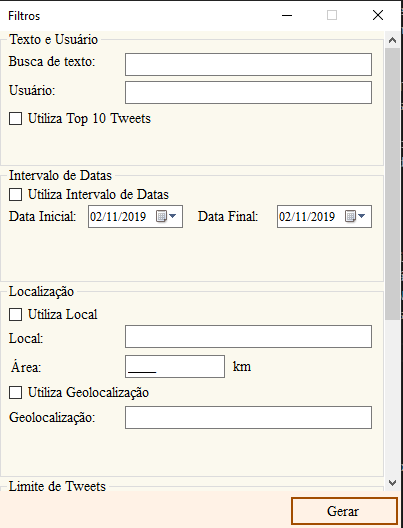
\includegraphics[width=10cm]{imagens/TwitterSearch.png}
\caption{Parte da tela principal do sistema}
\label{fig:TwitterSearch}
\end{figure}

Essa tela apresenta os dados do formulário referente a:

\begin{itemize}
\item Texto e Usuário:

\begin{itemize}
\item Busca de Texto: Essa busca irá filtrar no Twitter publicações que, em seu conteúdo, tenham a palabra digitada. Vale ressaltar que essa palavta será comparada de forma limpa e completa, ou seja, o texto para ser considerado igual deve ter a mesma palavra em seu conteúdo, não apenas parte dela.
\item Usuário: Irá pesquisar na rede social publicações do usuário digitado. Esse usuário é o nome que o mesmo utiliza na rede.
\item Utiliza Top 10 Tweets: Essa opção selecionará os Top 10 tweets do usuário digitado na opção anterior. Esse top 10 significa os 10 tweets mais importante daquele usuário, ou seja, os que faram mais retweetados e curtidos.
\item Usuário: Irá pesquisar na rede social publicações do usuário digitado. Esse usuário é o nome que o mesmo utiliza na rede.
\end{itemize}

\item Intervalo de Datas

\begin{itemize}
\item Utiliza Intervalo de datas: Essa opção ativa o intervalo de datas. Se selecionada, o sistema irá filtrar a data da pubicação do tweet no intervalo das datas selecionadas nos combos.
\item Data Inicial: Data inicial a se considerar os tweets do filtro. A data inicial é incluída no filtro também, ou seja, tweets publicados no dia selecionado também serão retornados.
\item Data Final: Data final a se considerar os tweets do filtro. A data final é incluída no filtro também, ou seja, tweets publicados no dia selecionado também serão retornados.
\end{itemize}

\item Localização

\begin{itemize}
\item Utiliza Local: Essa opção atia o filtro de localização onde o tweet foi publicado. Essa opção não considera a localização do usuário que postou o tweet, mas sim a localização que estava no momento que que foi publicado.
\item Local: Esse filtro pode considerar cidade, estado, país ou mesmo região. Um exemplo de utilização seria: Berlin, Germany.
\item Área: Perímetro a se considerar a partir do local selecionado. Uma opção de entrada seria 50km, então utilizando a opção anterior, de Berlin, esse filtro contataria até 50km em volta dessa cidade. 

\item Utiliza Geolocalização: Essa opção permite que o usuário utiliza geolocalização para filtrar os tweets. assim como o Local, a geolocalização irá identificar a partir do local em que o tweet foi publicado.
\item Geolocalização: Entrada de latitude e longitude. Um de entrada exemplo seria: 55.75, 37.61. A Área, já mencionada, também funciona se preenchida assim como a geolocalização.
\end{itemize}

\end{itemize}

Essa é a primeira tela do sistema. Esses filtros colocados são os principais e comumente mais utilizados. O trabalho \citeonline{Sabottke2015} utiliza filtro de texto e data para obtenção dos resultados. Em sua pesquisa, os dados têm por base o ano de 2015 filtrando a palabra CVE, que é a sigla utilizada para filtro de vulnerabilidades \cite{CVE1985}.

A figura \ref{fig:TwitterSearch2} apresenta a segunda parte da tela principal do sistema. Como o número de filtros é grande, o sistema acaba tendo uma barra de rolagem que disponibiliza o restante dos filtros.

\begin{figure}[H]
\centering
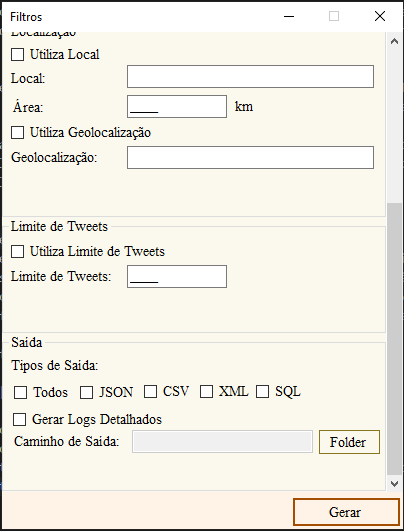
\includegraphics[width=10cm]{imagens/TwitterSearch2.png}
\caption{Segunda Parte da tela principal do sistema}
\label{fig:TwitterSearch2}
\end{figure}

A sequnência da tela apresenta os dados do formulário referente a:

\begin{itemize}

\item Limite de Tweets

\begin{itemize}
\item Utiliza Limite de Tweets: Essa opção valida se vai limitar o número de tweets no retorno da bucsa.
\item Limite: Número de Tweets máximo de retorno da consulta
\end{itemize}

\item Saída

\begin{itemize}
\item Tipos de Saída: Essa opção seleciona qual o tipo de saída do programa: JSON, CSV, XML, SQL.
\item Gerar Logs Detalhados: Essa opção faz com que os sistemas gerem um log detalhado sobre suas atividades.
\item Caminho de Saída: Essa opção permite que o usuário selecione onde os arquivos de saída devem ser copiados.
\end{itemize}

\end{itemize}

Esse sistema é a primeira parte do trabalho, cujo objetivo é apenas apresentar o formulário e, a partir do preenchimento dele, gerar um arquivo JSON de configuração de filtro de entrada para os outros arquivos.
 
\subsection{Tweet}

Esse sistema foi desenvolvido em Python e tem o objetivo de fazer a conexão com a API do GetOldTweets \cite{Pythoncommunity}. Para sua execução, ele precisa de um arquivo de entrada que contenha as informações dos filtros que será colocado na busca dos tweets. A imagem \ref{fig:entradaTweet} mostra um exemplo de um arquivo de entrada desse sistema.

\begin{figure}[H]
\centering
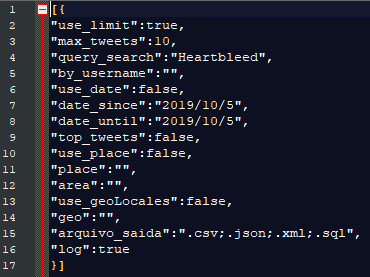
\includegraphics[width=8cm]{imagens/entradaTweet.png}
\caption{Exemplo de entrada do programa Tweet}
\label{fig:entradaTweet}
\end{figure}

Esses filtros são os enviados ao GetOldTweets\cite{Pythoncommunity} para obter o retorno. Desse retorno, para cada tweet x de resultado, é buscado o TOP 10 dos tweets referente àquele usuário que publicou o tweet x.

O sistema conta ainda com a opção de log, na figura \ref{fig:entradaTweet} apresentado na tag "log". Essa opção faz com que cada passou do sistema seja relatado em um arquivo de log no caminho: raiz da aplicação/log/"data do log". Essa opção é importante, pois nem sempre a API está funcionando corretamente, o que faz com que o sistema apresente lentidão em sua execução. 

Ademais, o sistema faz uma interação com o usuário afim de apresentar em qual parte da análise está sendo efetuada, conforme imagem \ref{fig:TweetExecucao}.

\begin{figure}[H]
\centering
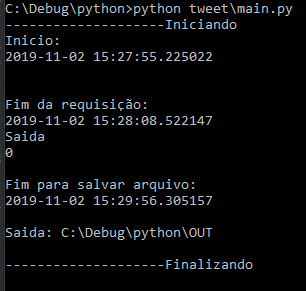
\includegraphics[width=8cm]{imagens/TweetExecucao.png}
\caption{Exemplo de execução do sistema Tweet}
\label{fig:TweetExecucao}
\end{figure}

O sistema apresenta a data e hora de início da execução. Após isso ele começa a realizar a requisição da API, quando finalizado apresenta a data e hora de finalização requisição. Após isso o Tweet chama a aplicação APIConectorJson, que faz o tratamento dos dados, quando finalizado apresenta data e hora da finalização do taratamento dos dados. Apresenta ainda a saída da requisição: 0 para sucesso e qualquer outro para código de erro do sistema operacional. No final apresenta o caminho onde os arquivos foram salvos.

O sistema funciona então em duas fases: (1) seleciona os filtros no arquivo de entrada e faz a requisição com a API gerando um arquivo de saída X e (2) seleciona esse arquivo de saída e chama o aplicativo APIConectorJson passando o arquivo X como entrada e passando quais são os tipos de saída desejados. 

\subsection{API GetOldTweets}

A API do GetOldTweets é uma biblioteca desenvolvida em python que tem o objetivo de fazer uma busca no Twitter apartir dos filtros possíveis, que serão descritos posteriormente. Seu funcionamento se baseia na leitura de um brownser que acessa a rede social, então o resultado é obtido a partir dessa busca. Logo, o resultado sempre fica ordenado de forma cronológica, ou seja, pela data da publicação.

Essa API possui vários recursos para ser utilizado, não se limitando apenas à uma bilioteca. É possível acessa-la através de linha de comando pelo CMD passando os parâmetros de busca, assim como é possível chama-la a partir de um programa externo, seja em python ou não. Cada uma das formas de chama-la gera um resultado diferente: se chamado por linha de comando é gerado um arquivo CSV com as informações, já chamando a partir de um programa externo a bilioteca retorna um arquivo JSON com os tweets. A estrutura dos objetos de retorno é dada com os seguintes atributos:

\begin{itemize}
\item id (string); Código referente ao tweet
\item permalink (string); Link da publicação
\item username (string); Nome do usuário que fez a publicação
\item text (string); Texto do tweet
\item date (datetime); Data da publicação
\item retweets (integer); Número de vezes que o tweet foi retweetado
\item favorites (integer); Número de vezes que o tweet foi favoritado
\item mentions (string); Lista as menções da publicação
\item hashtags (string); Apresneta as hashtags da publicação
\item geo (string); Localização onde o tweet foi publicado
\end{itemize}

Para o presente trabalho foi escolhido utilizar a API como uma biblioteca de um sistema externo, então é conectado na API e retornado o arquivo JSON com os dados da busca. 

A biblioteca funciona em duas partes: listar os filtros para a busca (classe TwitterCriteria) e realizar a busca propriamente dita (TweetManager). A classe de organização das buscas possui os seguintes métodos que possibilitam a realização dos filtros:

\begin{itemize}
\item setUsername (str or iterable): Nome do usuário para a busca
\item setSince (str. "yyyy-mm-dd"): Data de início da busca. Se não for dado um valor não há limite de busca. Se setado um valor esse é incluído no resultado, ou seja, se colocado a data 2015-01-01 no resultado haverá tweets dessa data.
\item setUntil (str. "yyyy-mm-dd"): Data final da busca. Se não colocado a data final será o dia em que a busca foi realizada, com resultados incluindo esse dia. Se setado o dia colocado não é considerado no resultado, ou seja, se colocado 2015-12-31 não haverá tweets dessa data.
\item setQuerySearch (str): Texto para verificação no Twitter. Esse texto será buscado na rede como um todo e deve haver um "match" completo da palavra para o tweets ser considerado resultado da busca. Ou seja, se filtrado a palavra "CVE", como será feito por esse trabalho, será retornado todos os tweets da rede que tenham essa palavra. A busca não é case sensitive, ou seja, não importa texto em maiúsculo e minúsculo.
\item setTopTweets (bool): Se setado como "true" é retornado apenas os Top tweets. Esse conceito de Top tweet se baseio no número de curtida e número de seguidores do usuário que publicou o tweet.
\item setNear(str): Uma referência de área localização onde o tweet foi publicado. 
\item setWithin (str): Filtra a busca por uma área de localização a partir da opção colocada no setNear.
\item setMaxTweets (int): O número máximo de tweets a ser suportado na busca dos dados. Se não setado ou se o valor for menor que 1 será retornado a busca total dos tweets, sem limite.
\end{itemize}

A biblioteca possui ainda algumas limitações baseada nas condições em que a busca é efetuada. Basicamente, se a rede for oscilante no momento de leitura e requisição dos dados é possível que o retorno não seja composto por todos os tweets da busca, uma vez que a API faz uma busca na rede social lendo um brownser, ou seja, se não carregar os dados no navegador a biblioteca não terá nada para ler, ou se carregar apenas parte irá retornar apenas esse trecho de resultado. Para facilitar a busca de ocorrência desse problema basta conferir no resultado a data do último tweet retornado, se a data for uma não reconhecida, ou seja, não for a desejada, houve erro na busca. Esse erro também pode ocorrer devido ao estouro da memória principal, pois a API faz a busca utilizando dessa memória para armazenamento dos dados para apenas depois montar o arquivo de saída.

Para o presente trabalho foi enfrentado ambos os problemas. Como será citado nos resultado, a busca foi feita para o ano de 2019, mas comparando aos resultados dos anos anteriores (2018, 2017, 2016 e 2015), e para a busca de todo esse período foi encontrado certa dificuldade por limitação de rede e de memória.

\subsection{APIConectorJson}

Essa parte do sistema funciona com o propósito de organizar as informações obtidas da API GetOldTweets \cite{Pythoncommunity}. Ele recebe de entrada um arquivo JSON com os dados da requisição e recebe também quais são as saídas esperadas conforme citado na seção anterior. Desse arquivo é retirado todos os objetos e para cada um dos tipos de saída é feito um tratamento diferente. Além disso, todo o processo também pode ser logado caso haja alguma espécie de erro. Esse log é o mesmo do sistema Tweet.

Os tipos de saída são configurados da seguinte forma:

\begin{itemize}
\item JSON: Arquivo com estrutura pré estabelecida, é um modelo para armazenamento e transmissão de informações no formato texto e que é bastante utilizado por aplicações Web que trabalham com a tecnologia AJAX. É um objeto JavaScript. A própria API do GetOldTweets \cite{Pythoncommunity} retorna o arquivo JSON com o resultado, então o sistema só copia o arquivo para a pasta de saída.  
\item CSV: Arquivo com a estrutura de informações separados por vírgulas. Comunmente utilizado para apresentação de informações em planílhas e cópias de dados entre bases de informações, como banco de dados. Esse tipo de armazenamento agrupa as informações de texto em planilhas. O sistema o utiliza colocando os tipos na primeira linha do arquivo e as informações nas demais.
\item XML: é um tipo de armazenamento que utiliza a linguagem de marcação recomendado pela W3C. É utilizado para representação de dados de forma estruturada mantendo as informações de acordo com suas especificidades. Utiliza de tags para caracterizar uma informação. O sistema utiliza as tags colocando os tipos dos dados nelas e a informação no espaço restante.
\item SQL: é um armazenamento em banco de dados comum, tabelado. A informação é colocada em uma tabela onde a coluna é o tipo de informação e as linhas são as tuplas de informações. O sistema utiliza esse tipo colocando os tipos dos tweets como as colunas da tabela RETORNO e as linhas são os tweets que estavam no arquivo JSON de entrada.
\end{itemize}

O sistema então tem como objetivo organizar os dados do arquivo de entrada nos aruqivos de saída. Ele trabalha apenas com essa função, possibilitando que qualquer arquivo de entrada JSON tenha sua saída nos tipos permitidos de dados: JSON, CSV, XML e SQL. 

\subsection{Scanner}

O conjunto dos sistemas anteriormente citados dá origem ao sistema Scanner. Esse possui a interface do TwitterSearch, o que possibilita preenchimento do formulário disponibilizando um arquivo JSON de configuração de filtragem e que chama o "cérebro" do programa: o Tweet. Este processa o arquivo de entrada com os filtros requisitando a API GetOldTweets \cite{Pythoncommunity} com esses dados, obtendo os tweets de retorno que satisfazem a busca, criando um novo arquivo json de saída contendo uma lista com os objetos dos tweets retornados pela API. Assim chama o APIConectorJson para organização dos dados passando o JSON com os objetos dos tweets e passando os tipos de saída selecionado no TwitterSearch, depois de finalizado o próprio Tweet copia as saídas para o caminho selecionado pelo usuário.

Um exemplo de funcionalidade segue na figura \ref{fig:entrada1} que apresenta as seguintes entradas.

\begin{figure}[H]
\centering
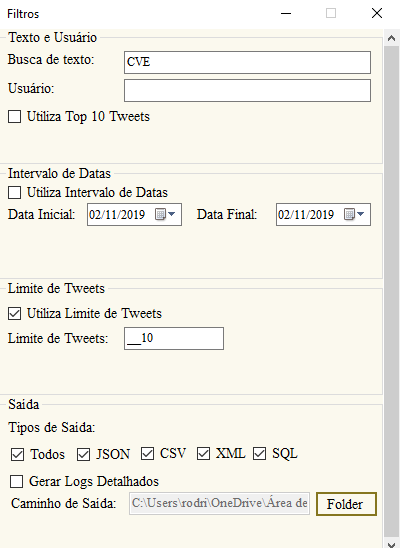
\includegraphics[width=10cm]{imagens/entrada1.png}
\caption{Entrada de exemplo (imagem editada com o propósito de listar apenas os filtros utilizados)}
\label{fig:entrada1}
\end{figure}

Com essas estradas, o sistema chama as outras aplicações e obtem as saídas nos arquivo em JSON, CSV, XML e SQL. Todos esses arquivos possuem os dados de retorno do Twitter com a busca feita. Tomando como exemplo um desses tweets do retorno da busca, o de ID 1190312935895158789 do usuário Tribe\_Secure, ele é listadas nas figuras \ref{fig:saidaJson}, \ref{fig:saidaCSV}, \ref{fig:saidaXML} e \ref{fig:saidaSQL}.

\begin{figure}[H]
\centering
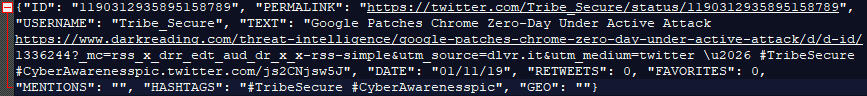
\includegraphics[width=1\textwidth]{imagens/saidaJson.png}
\caption{Exemplo do tweet em saída JSON (o texto foi alinhado para uma melhor visualização)}
\label{fig:saidaJson}
\end{figure}

\begin{figure}[H]
\centering
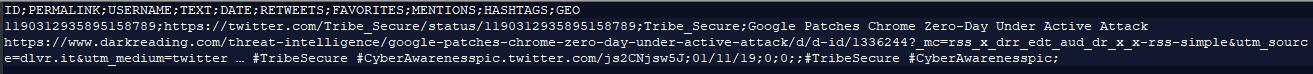
\includegraphics[width=1\textwidth]{imagens/saidaCSV.png}
\caption{Exemplo do tweet em saída CSV}
\label{fig:saidaCSV}
\end{figure}

\begin{figure}[H]
\centering
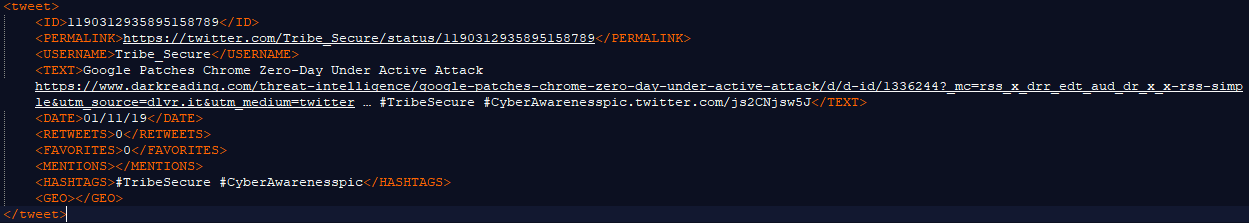
\includegraphics[width=1\textwidth]{imagens/saidaXML.png}
\caption{Exemplo do tweet em saída XML}
\label{fig:saidaXML}
\end{figure}

\begin{figure}[H]
\centering
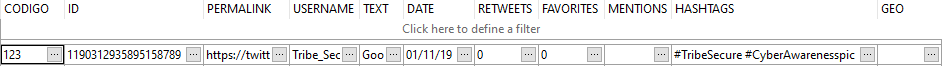
\includegraphics[width=1\textwidth]{imagens/saidaSQL.png}
\caption{Exemplo do tweet em saída SQL}
\label{fig:saidaSQL}
\end{figure}

O exemplo de entrada ainda será utilizado nesse trabalho, filtrando ainda por data. Como o retorno monta uma base de dados consideravelmente grande, ele já mostra que o volume de dados de quando não se coloca limite de número de tweets pode crescer ainda mais. A fim de teste, foi colocado uma busca com um número ilimitado de tweets e sem fechar nenhuma data, como resultado passaram-se mais de 24 horas e o programa ainda não tinha finalizado suas solicitações.

Esse é o sistema no qual o trabalho se baseia. É com ele que a análise sobre as quantidade de vulnerabilidades discutidas no Twitter será possível, assim como a frenquência da mesma nos últimos anos. Esse é um programa genérico que possibilita buscas em toda a rede, logo será nossos filtros que farão com que a busca seja orientada aos objetivos do trabalho.

\subsection{FindWords}

Esse sistema tem como objetivo buscar uma palavra (ou parte dela) em arquivos de diretórios distintos. Dado um diretório A e a palavra "CVE", o programa irá listar como resultado todos os arquivos da pasta e subpasta do diretório A que conténham essa palavra e em qual linha do arquivo a mesma está. 

O objetivo desse programa é buscar para cada resultado do Scanner o código CVE publicado nas listas presente no site NVD. A partir desse resultado é possível verificar quais vulnerabilidades estão sendo discutidas e realmente existem no cite do CVE e do NVD.

O programa possibilita ler todos os possíveis arquivos de saída do Scanner (XML, JSON, CSV e SQL) e, a partir desses arquivos, ler o código descrito na publicação no Twitter e buscar esse código nas bases de conhecimento do NVD.

O resultado dessa busca é um arquivo txt de saída que lista o código CVE encontrado no tweet e o diretório do arquivo e linha do arquivo em que o mesmo código foi encontrado.

Há ainda a possibilidade de, ao invés de procurar nos arquivos do diretório selecionado, utilizar um banco de dados para a busca da palavras.

\section{Coleta de dados}

O Scanner faz uma busca no Twitter a partir da API GetOldTweets \cite{Pythoncommunity} passando os parâmetros de filtro. Essa é a coleta de dados que o sistema faz da rede social. 

Para trabalhar com os dados, eles são organizados em outros arquivos que possibilitam a visualização melhor dos dados, assim o trabalho de análise fica mais simples.

O site do NVD, como já foi citado, apresenta uma lista de opção para download das vulnerabilidades. O site organiza essas informações colocando-as em um arquivo ZIP para cada ano \cite{NISTDownload}. Assim, é possível baixar essas informações e utilizar delas para analisar os dados de retorno. O site do CVE também fornece a opção de baixar o um arquivo XML com os mesmos dados, mas o arquivo não é em formato ZIP e acaba sendo um pouco maior para download \cite{TheMITRECorporation2018}.

A coleta de dados então é feita a partir de duas bases para a análise desse trabalho: Twiiter, através da API do GetOldTweets \cite{Pythoncommunity}; e o NVD, que processa seus dados a partir da base do CVE.

Tomando como exemplo a figura \ref{fig:exemploVulnerabilidade}, tem-se a vulnerabilidade de código CVE-2019-2110. A figura \ref{fig:exemploVulnerabilidadeCVE} apresenta suas informações no site do CVE.

\begin{figure}[H]
\centering
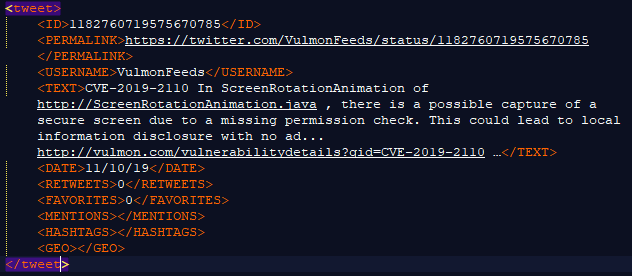
\includegraphics[width=1\textwidth]{imagens/exemploVulnerabilidade.png}
\caption{Exemplo de publicação de uma vulnerabilidade no Twitter em formato xml}
\label{fig:exemploVulnerabilidade}
\end{figure}

\begin{figure}[H]
\centering
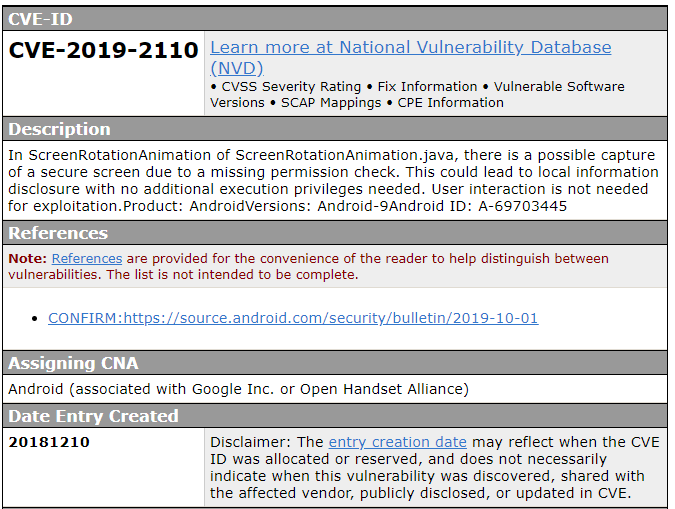
\includegraphics[width=1\textwidth]{imagens/exemploVulnerabilidadeCVE.png}
\caption{Descrição da vulnerabilidade CVE-2019-2110 no site do CVE \cite{CVE1985}}
\label{fig:exemploVulnerabilidadeCVE}
\end{figure}

O arquivo disponibilizado no site do NVD referente ao ano de 2019 descreve a vulnerabilidade, como apresentado na figura \ref{fig:descricaoVulnerabilidadeNVD}. Assim como o arquivo XML baixado no site do CVE, apresentado na figura \ref{fig:descricaoVulnerabilidadeCVE}.

\begin{figure}[H]
\centering
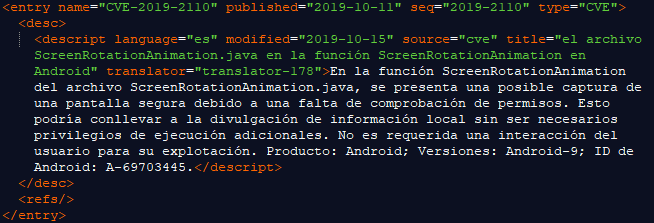
\includegraphics[width=1\textwidth]{imagens/descricaoVulnerabilidadeNVD.png}
\caption{Descrição da vulnerabilidade CVE-2019-2110 no arquivo disponibilizado no NVD}
\label{fig:descricaoVulnerabilidadeNVD}
\end{figure}

\begin{figure}[H]
\centering
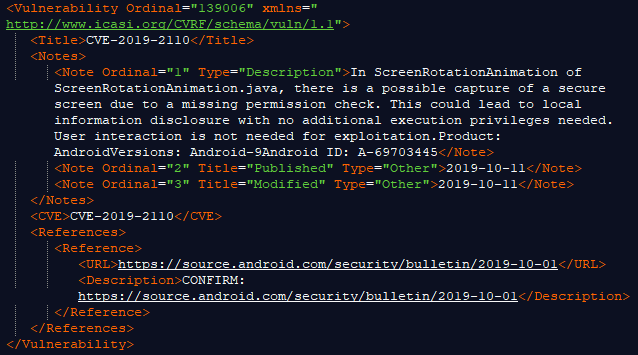
\includegraphics[width=1\textwidth]{imagens/descricaoVulnerabilidadeCVE.png}
\caption{Descrição da vulnerabilidade CVE-2019-2110 no arquivo disponibilizado no CVE}
\label{fig:descricaoVulnerabilidadeCVE}
\end{figure}

A coleta dos dados então não se restringe apenas ao Twitter, mesmo que o objetivo seja a verificação de discussão sobre vulnerabilidades na rede social. A coleta é feita nos sites que tratam de vulnerabilidades para a identificação correta do que é ou não vulnerabilidade. Parte da análise está em filtrar na rede social, a outra está na identificação dessas vulnerabilidades.

Para o presente trabalho os filtros foram feito para esse ano (o objetivo é identificar como a discussão está hoje!). Logo, tanto no site do NVD quanto no CVE foi baixado os arquivos referente ao ano de 2019 e os mesmos serão utilizados em conjunto com o filtro feito de publicações do ano de 2019 por parte do Scanner.

Então o Scanner é o responsável por buscar esses dados do Twitter e o FindWords será o responsável por relacionar os dados recolhidos da rede social com os dados presentes nos sites do CVE e do NVD.

No próximo capítulo será listado os resultados dessas buscas comparando outros anos. O número de vulnerabilidades tem crescido exponencialmente, isso é fato, o CVE prova isso a partir dos tamanhos dos arquivos de cada ano. Esse aumento também é experado no número de pessoas discutindo o tema no Twitter. 

